%!TEX root = ../main.tex

\chapter{Transcription}\label{ch:transcription}

This chapter is dedicated to the problem of offine handwriting recognition, that is, given an image of a text line, find the corresponding characters and words. Although some may consider it a solved task, since many approaches achieve very good performance on a wide variety of corpora (see \autoref{sec:related_transcription}), we remind the reader that our use case poses several challenges that are not present in the controlled environments of academic contests (\autoref{sec:challenges}). Of these, we summarise the most important ones:
\begin{description}
	\item[unbefitting writing conditions] The documents are completed in a rush, soon after an accident, with no proper support structure for writting and with few format restrictions.

	\item[unconstrained recognition] Statements include text which does not admit a vocabulary for correction, such as phone numbers and license plates.

	\item[lack of annotated data] As in the case of detection, we started the project having only a database of images and no useful annotations.
\end{description}

The chapter first introduces the \CRNN{} architecture \citep{CRNN}, which has become almost a standard for optical character recognition in the recent years. Then, \autoref{sec:transcription_experiments} presents several experiments for training, including various methods of data generation. Each new experiment tries to address the weaknesses of the previous one, in a quest of reproducing the great results obtained on clean handwriting databases and in OCR. Finally, we present an overview of the obtained results in \autoref{sec:transcription_results} and why our observations prove this problem is more difficult than OCR.



%========================================================================================

\section{Convolutional Recurrent Neural Networks}\label{sec:crnn}

	%--INTRO --------------------------------------------------------------------------------

		Text transcription has preoccupied researchers for a very long time. Therefore, a large amount of ideas have been tried in order to solve this problem, of which we mention a few in \autoref{sec:related_transcription}. One of the challenges of text resides in its wide variation of appearance. For example, a free font website such as \url{www.1001fonts.com/} currently lists approximately 9500 different typefaces. Moreover, it is believed that each person has a completely unique handwriting, which is why this is still commonly used a signature. This highlights the importance of being able to represent images of text robustly, or, in other words, to extract good features that distinguish well among characters. As was previously stated, convolutional neural networks have proved very effective in this task time and again, so it is natural to use them as a first stage in a transcription architecture.

		Another peculiarity of text, which we have also mentioned in the detection chapter, is given by its sequential aspect. Few neural network architectures support arbitrarily-sized input. Of these, the recurrent neural network (RNN) has become a standard since it models well sequences of any type.

		The Convolutional Recurrent Neural Network (\CRNN{}) architecture uses the two approaches above in a unified framework to transcribe text from natural images. Considering that it achieved state-of-the-art performance in such a challenging task, we believe it is suitable for our use case as well, which is why we focused most of our efforts in this direction. Next, we detail its inner workings as they are crucial in devising our experiments.


		\begin{figure}
		\begin{subfigure}[c]{.48\linewidth}
		\begin{flushleft}
		\footnotesize
		\begin{tabular}{|l|c|}
			% \footnotesize
			\hline
			\textbf{Type} & \textbf{Configurations}						\tabularnewline	\hline
																																				\hline
			Transcription & - 																\tabularnewline	\hline
			Bi-LSTM & \#hidden units:256						\tabularnewline	\hline
			Bi-LSTM & \#hidden units:256						\tabularnewline	\hline
			Map-to-Seq & - 															\tabularnewline	\hline
			BatchNorm & - 														\tabularnewline	\hline
			Conv (7) & \#maps:512, k:$2\times2$, s:1, p:0	\tabularnewline	\hline
			MaxPool (4) & Window:$1\times2$, s:2								\tabularnewline	\hline
			Conv (6) & \#maps:512, k:$3\times3$, s:1, p:1	\tabularnewline	\hline
			BatchNorm & - 														\tabularnewline	\hline
			Conv (5) & \#maps:512, k:$3\times3$, s:1, p:1	\tabularnewline	\hline
			MaxPool (3) & Window:$1\times2$, s:2 							\tabularnewline	\hline
			Conv (4) & \#maps:256, k:$3\times3$, s:1, p:1	\tabularnewline	\hline
			BatchNorm & - 														\tabularnewline	\hline
			Conv (3) & \#maps:256, k:$3\times3$, s:1, p:1	\tabularnewline	\hline
			MaxPool (2) & Window:$2\times2$, s:2								\tabularnewline	\hline
			Conv (2) & \#maps:128, k:$3\times3$, s:1, p:1	\tabularnewline	\hline
			MaxPool (1) & Window:$2\times2$, s:2 							\tabularnewline	\hline
			Conv (1) & \#maps:64, k:$3\times3$, s:1, p:1		\tabularnewline	\hline
			Input & $W\times32$ gray-scale image 							\tabularnewline	\hline
		\end{tabular}\par
		\caption[\CRNN{} structure]{\todo{Note different from paper, use tabu, split conv part separately }}\label{fig:crnn_architecture}
		\end{flushleft}
		\end{subfigure}
		\begin{subfigure}[c]{.49\linewidth}
			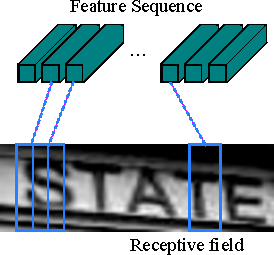
\includegraphics{crnn_rec_field}
			\caption{Image encoding into sequence of features \citep[credit to][]{CRNN}}\label{fig:crnn_sequence}
		\end{subfigure}
		\caption{The \CRNN{} architecture}
		\end{figure}

	%----------------------------------------------------------------------------------------
	\subsection{Feature extraction}
		The first part of the \CRNN{} architecture consists of a custom 7-layer CNN that transforms the input image into a sequence of high-level features. This is similar to well-known architectures, as it alternates convolutional and pooling layers (\autoref{fig:crnn_architecture}). A few particularities are important to be noted.

		First, the input is pooled differently on the vertical dimension than on the horizontal one. For the former, 4 layers with pooling windows of height 2 are used. As a result, an input of height 32 becomes a feature map of height 2. This is further reduced this to a \(\mathit{height} = 1\) feature by the last convolutional layer, which applies \(2 \times 2\) convolution with no padding. For the horizontal direction, the nework performs pooling only twice with a window of width 2. This ensures the receptive field does not become too wide and can still distinguish very narrow characters such as \{\texttt{l,i,1}\}. The network is fully convolutional, which allows inputs of any size to be processed. However, since the columns become features of the RNN, the height should be standardised. This design is well suited for images of text which are bounded vertically, but not horizontally.

		Second, the network uses batch normalisation \citep{batch_norm}, which is standard practice in recent times since it improves the performance and the stability of the network. This works by replacing the activations \(\ve{H}\) of a layer with their normalised counterparts \(\ve{H}'\), which become the new inputs for the next layer: \[
			\ve{H}' = \gamma \frac{\ve{H} - \ve{\mu}}{\ve{\sigma}} + \beta,
		\]\footnote{\todo{make miu and sigma vectors}} where \(\mu\) is a vector of means of all neurons and \(\sigma\) a vector of their standard deviations. The learnable parameters \(\gamma\) and \(\beta\) ensure the network does not lose expressive power by allowing convergence towards any mean and standard deviation. Overall, using this technique means that the composition of the batches is important, as we will see shortly.

		Finally, we use ReLU activations at each layer and bias terms for the convolution.

		%........................................................................................
		\subsubsection*{Input preprocessing}

			Input images are resized to have a heigth of 32px, while keeping their aspect ratio. As a result, their widths are different which makes it difficult to construct batch tensors. Therefore, we also define a standard input width of 250px and make sure all training images are narrower than this in the interest of avoiding horizontal deformation. Images that are shorter than the necessary width are duplicated horizontally up to this size. As opposed to padding the shorter images with blank space, this concatenation mechanism keeps a similar distribution of pixels across all batches. Note this does not produce bad training examples because we keep track of the original length when aligning the predictions and the labels.

	%----------------------------------------------------------------------------------------

	\subsection{RNN decoder}\label{sec:LSTM}
		The CNN part of the architecture encoded horizontal portions of the image (of full height) into a sequence of high dimensional features, ordered left to right (\autoref{fig:crnn_sequence}). This sequence is then consumed by an RNN decoder in order to produce character representations. To avoid the problem of vanishing gradients in long sequences, the LSTM version is employed \citep{LSTM_original} which uses a combination of gates to control the flow of information inside the cell. By default, an LSTM cell can only use past context in addition to the current input. In our case, future context can be very helpful, so a bi-directional variant of LSTM is used. 	Moreover, using a stack of two such layers allows us to capture more complex contextual dependencies.

		%........................................................................................
		\subsubsection*{Connectionist Temporal Classification}\label{sec:CTC}

			Training RNNs normally requires ground truth labels at each time step. We can see this is problematic in our context, since we only know the final sequence and not how it is aligned to the input image. Moreover, some features in the sequence can correspond to space between the characters, so there is no ground truth for them.

			This problem is solved using the Connectionist Temporal Classification method \citep[CTC; ][]{CTC}. It requires the output of the network to be a softmax output layer with \(N + 1\) units, \(N\) being the size of our alphabet \(L\). Each unit represents the probability of a symbol in the alphabet, and the extra unit corresponds to observing no label, which is denoted by ``\(-\)'', a \emph{blank} symbol . In this way, the outputs define the probabilities of all possible alignments of the input sequence with all possible output sequences.

			Additionally, the method requires a many-to-one mapping function from sequences of network outputs, denoted as \(\pi\), to actual labels, denoted as \(\bm l\): \[
				\mathcal{B}: L'^T \to L ^{\leq T},~L' = L \cup \{-\},
			\] where \(L^{\leq T}\) is the set of all possible sequences of length up to \(T\).
	 		For example, \(\mathcal{B}\) maps \mbox{$\pi$: ``\texttt{$-$fee$-$mmm$-$mm$--$ee$-$}}'' to $\bm l$:  ``\texttt{femme}'' by removing duplicates and blanks. Note that the order of these operations is important; removing blanks first results in impossibility of mapping double characters.

	 		Finally, CTC defines the probability of a given label \(\bm{l} \in L^{\leq T}\) conditioned on the input sequence \(\mathbf{x}\) as the sum of the probabilities of all output paths \(\pi\) that correspond to it:
	 		\begin{align*}
				p(\bm{l} | \bm{x}) &= \sum_{\pi:{\cal B}(\pi)=\bm{l}}p(\pi|\bm{x}), \\
				p(\pi | \bm{x}) &= \prod_{t=1}^T \bm{y}_{\pi_t}^{t},
				\label{eq:stringprob}
			\end{align*}
			where \(\bm{y}_{\pi_t}^{t}\) is the probability of observing label \(\pi_t\) at time \(t\), as outputted by the network.

			Given the exponential number of possible sequences \(\pi\) corresponding to \(\bm l\), finding the most probable label \(h(\bm{x}) = \argmax_{\bm{l} \in L^{\leq T}} p(\bm{l} | \bm{x})\) for an input \(\bm x\) becomes intractable very quickly. Therefore, an approximation is made based on the assumption that the most probable path will correspond to the most probable labelling:\[
				h(\bm{x}) \approx \mathcal{B}(\pi^*),~~ \text{where } \pi^* = \underset{\pi}{\argmax}~ p(\pi|\bm{x}).
			\] Decoding in this way can be calculated either with the backward-forward algorithm, or greedily with beam search.

			The loss function between a predicted labelling \(h(\bm{x})\) and a target ground truth label \(\bm z\) is calculated as the edit distance between the two, i.e.\ the number of insertions, deletions or substitutions needed to transform one into the other.

	%----------------------------------------------------------------------------------------

	\subsection{Training and evaluation}
		An input image flows through the convolutional layers and into the LSTM ones, whose predictions are aligned with the ground truth text as explained above. This allows the network to be trained end-to-end on pairs of images and sentences, with the error being back-propagated through all layers. In particular, the LSTM layers use Truncated Back-Propagation Through Time. Also, we noticed improvements when using dropout on the output of the final LSTM with a dropping probability \(p_\mathit{drop} = 0.2\).

		We train the network on batches of 512 images using the Adam optimiser \citep{adam} with a learning rate \(\alpha = 0.001\) and exponential decay rate for the first moment estimates \(\beta_1 = 0.5\). We also tried using an exponentially decreasing learning rate, but found it counterproductive since it needed tuning for each individual corpus or else it would slow down the learning before reaching a plateau.

		Finally, we used an alphabet of 81 characters that we identified in the corpus of the RIMES database: \(2 \times 26\) lower and upper-case letters, 10 digits, 13 French-specific letters with diacritics, and 6 symbols. In addition, we set the architecture to treat as errors differences regarding the case of letters during train time. It is important to note, though, that the distribution of characters in a corpus is not equal, as it is a feature of the language.

		%........................................................................................
		\subsubsection*{Evaluation}
			As in the case of text detection, we started with no ground truth labels on real data. Therefore, to have an objective and relevant measure of the models' performance, we also annotated the bounding boxes of the \ds{Test} dataset. However, the quality for some of these prevented us from providing an accurate transcription. Therefore, we transcribed illegible glyphs with a placeholder character that is not part of the training set. This was done so as to allow wrong predictions at this point while providing normal evaluation for the legible part.

			Given the small size of the \ds{Test} dataset of only 1400 examples, no experiments used it either for training or validation. Each model was only evaluated once on this dataset, and we recorded its performance.

			We use the \emph{normalised} character error rate (CER), and the word error rate (WER) for measuring the performance of different models, expressed as percentages: \[
			\begin{aligned}
				\cer &= \frac{100}{N} \sum_i \frac{\operatorname{dist}(\mathit{prediction}_i, \mathit{groundTruth}_i)}{\card{\mathit{groundTruth}_i}},\\
				\wer &= \frac{100}{N} \sum_i (1 - \delta (\mathit{prediction}_i, \mathit{groundTruth}_i)),
			\end{aligned}
			\]
			where the \(\operatorname{dist}()\) function evaluates the edit distance and \(\delta\) outputs 1 if its arguments are the same, letter for letter, or 0 when they differ. Note that, unless otherwise specified, we use the raw values, without discounting for placeholders in the ground truth. This results in minimally attainable error rates that are slightly above zero: \(\cer_\mathit{min} = 0.8\%,~\wer_\mathit{min} = 5.02\%\).

			Normalising the CER by the length of ground truth is important for aggregating over multiple predictions. Otherwise, mistakes in shorter words would have a heavier contribution than those in longer words. In addition, normalisation also helps in getting an intuitive understanding of the measure; for example, \CER{33} means that one character in three is wrong.

	%----------------------------------------------------------------------------------------

%========================================================================================

\section{Experiments}\label{sec:transcription_experiments}
	Considering the lack of real training data, we try to achieve our goal by the means of transfer learning: we will train our models on several different datasets and evaluate them on real data. The rest of the section presents step-by-step our experiments, describing for each of them the training data, the performance of the model and the identified weaknesses.

	%----------------------------------------------------------------------------------------

	\subsection{Academic databases}
		%........................................................................................
		\subsubsection*{Datasets}
			At the very first phase, we validated that the architecture can learn and perform handwriting recognition by training on the already-discussed RIMES database. We trained and predicted using images of single words, hence the name \ds{Word} model. This converged after seeing \(\approx 780\)k training examples to a \emph{validation} \CER{8.29},	but it did not work on our documents, where \CER{115}. We realised again the importance of pixel values, so we re-trained on \emph{binarised} words (\ds{Word_bin} model), which performed similarly on validation dataset, but had a great improvement on \ds{Test}, with \CER{61.8}. Adding dropout with probability \(p_\mathit{drop} = 0.2\) further lowers the CER by 2\% (\ds{Word_bin_drop} model).

			\begin{figure}
				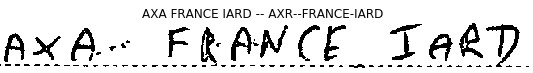
\includegraphics[width=.49\linewidth]{crnn/word_model_3}
				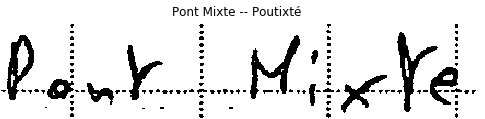
\includegraphics[width=.49\linewidth]{crnn/word_model_1}
				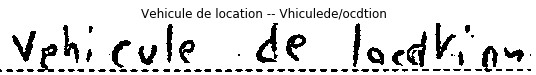
\includegraphics[width=.49\linewidth]{crnn/word_model_2}
				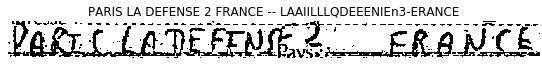
\includegraphics[width=.49\linewidth]{crnn/word_model_4}
				\caption[Predictions of \ds{Words_bin} model]{The ground truth and the predictions are shown above the images (left and right, respectively). When there are few background elements, the prediction works reasonably well, with the exception of missing spaces.}
				\label{fig:crnn_word_drop_model}
			\end{figure}

			We note that in the examples where the model almost works (\autoref{fig:crnn_word_drop_model}) some of the errors come from the model not being able to predict spaces. This is expected since there are no examples of it in the training set, which contains only images of full words. We try to correct this by including images of multiple words and spaces. However, we cannot use full lines due to their wildly varying widths, which become a problem for making training batches. Moreover, our cutting algorithm from \autoref{sec:rimes_template} cannot always produce accurate (\texttt{image},\texttt{text}) pairs due to inconsistencies in ground truth data. Therefore, we choose to add those lines from the RIMES database which are narrower than the input width (250px). Given that there are only a few of them, approximately 1000 compared to 50\,000 words, we decide to also add similarly short lines from the IAM handwriting database \citep{iam}, which adds appoximately 2500 examples. With these, together with the words images, we train a new model (\ds{Word_short_IAM}) which again achieves a similarly good performance on its validation dataset. Surprisingly though, it performs much worse on the statements, with a \CER{104}. We believe this is due to the additional English corpus from the IAM database which confuses the language model of the LSTM.

		%........................................................................................
		\subsubsection*{Outcome}
			The experiments on academic corpora revealed several key differences between them and the target dataset. One consists of the influence of pixel values (gray vs binary) and of background elements (\autoref{fig:crnn_dashes}), which increases validation CER from 17\% to 37\%. Another is given by the style of the handwriting: the one in RIMES database is mostly cursive, whereas IAM and the statements have more ``printscript'' style (using block letters). Then, the content is important too: we observe a consistent difference between strict and lowercase-only matching (\autoref{tab:transcription_academic}), meaning the model has trouble differentiating the case of words. Finally, we observe the great importance of the language model. Besides the problems introduced by using an English corpus, the continuous, gramatically-correct sentences in the RIMES database precondition the LSTM in a way that does not apply to the statements, whose fields are mostly names, addresses and numbers.

			In general, we validated through many small experiments that it is possible to learn to transcribe handwriting from our corpus by training on a different one. While the results so far are cannot be used in practice, the performance improvements demonstrate that transfer learning is a valid strategy, so we continue to explore it. In addition, we validate the results of \citet{MDLSTM_dropout}, showing that dropout consistently improves the performance. Therefore, all further models will use it, with \(p_\mathit{drop} = 0.2\).

			\begin{figure}
				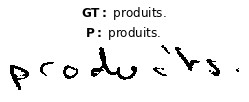
\includegraphics[width=.32\linewidth]{crnn/short_ok_1}
				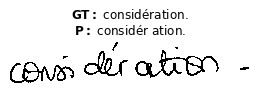
\includegraphics[width=.32\linewidth]{crnn/short_ok_2}
				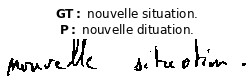
\includegraphics[width=.32\linewidth]{crnn/short_ok_3}
				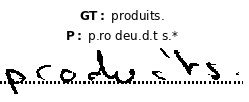
\includegraphics[width=.32\linewidth]{crnn/short_dash_1}
				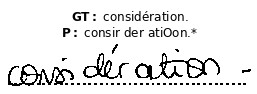
\includegraphics[width=.32\linewidth]{crnn/short_dash_2}
				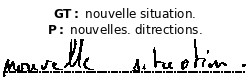
\includegraphics[width=.32\linewidth]{crnn/short_dash_3}
				\caption[Influence of backgrond elements]{The same model \ds{Word_bin_drop} was evaluated on clean images from RIMES (top) and their variants with added indicator line (bottom). This simple perturbation increases the error rate by \(20\%\). }
				\label{fig:crnn_dashes}
			\end{figure}

			\begin{table}
				\centering
				\begin{tabular}{| l | *{4}{c |}}\hline
					\textbf{Dataset name} & \textbf{CER strict} & \textbf{CER lower} & \textbf{CER ascii} & \textbf{WER}\\\hline
					\ds{Word} & 115.52 & 109.98 & 109.83 & 98.28\\
					\ds{Word_bin} & 62.43 & 59.44 & 59.43 & 94.25\\
					\ds{Word_bin_drop} & 60.58 & 57.71 & 57.71 & 94.83\\
					\ds{Word_short_IAM} & 104.19 & 100.24 & 100.15 & 98.78\\
					% \ds{Word_short} & 103.70 & 100.97 & 100.74 & 98.71\\
					\ds{Word_short_drop} & 103.77 & 100.36 & 100.17 & 97.70\\\hline
				\end{tabular}
				\caption[Academic datasets results]{Results of the \CRNN{} model trained on different datasets from the academic databases RIMES and IAM. Largely impractical, but useful to confirm the influence of various factors.}\label{tab:transcription_academic}
			\end{table}

	%----------------------------------------------------------------------------------------

	\subsection{Generator}\label{sec:generator}

		%... Description ........................................................................
			Inspired by the state-of-the-art achievements in OCR with synthetic data \citep{synthetic_data}, we try to address the limitations of the academic databases using a similar approach. Specifically, we adapt the code released by aforementioned authors to better suit our task by bringing the following improvements:
			\begin{description}
				\item[jiggle letters] Humans rarely have pixel-accurate alignment of their handwriting; likewise for the horizontal distribution of letters. Therefore, we randomly jiggle letters side-ways as well as up and down.

				\item[rotate, do not bend] As we noticed in the RIMES database, the baseline of handwriting is sometimes skewed from the horizontal. However, it is rarely bent. We reflect this in the generated text.

				\item[size and binarisation] Allow the generation of binarised text of specified height so as to avoid later resizing and its artefacts.

				\item[document-like noise] Add salt and pepper noise similar to that produced by optical scanners. Also add background elements such as randomly dashed indicator lines on text's baseline position.

				\item[real corpora and format] Generate real text based on publicly available datasets of person names, street and city names. Also generate according to various standard formats for dates, phone numbers and license plates.

				\item[cursive rendering] Allow rendering of fonts with ligatures to better resemble cursive handwriting.
			\end{description}

			\begin{figure}
				\setkeys{Gin}{height=16pt}
				\setkeys{Gin}{width=.5\ginnatwidth}
				% \setkeys{Gin}{width=.32\linewidth}
				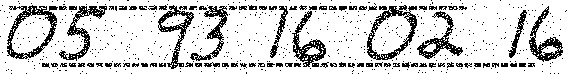
\includegraphics[width=6cm]{crnn/generated/987}\hspace{3mm}
				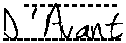
\includegraphics{crnn/generated/3}\hspace{3mm}
				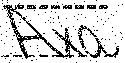
\includegraphics{crnn/generated/12}\\\vspace{3mm}
				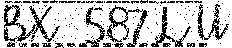
\includegraphics{crnn/generated/27}\hspace{3mm}
				
\includegraphics{crnn/generated/35}\hspace{3mm}
				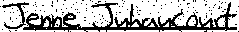
\includegraphics{crnn/generated/47}\\\vspace{3mm}
				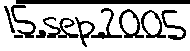
\includegraphics{crnn/generated/57}\hspace{3mm}
				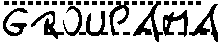
\includegraphics{crnn/generated/65}\hspace{3mm}
				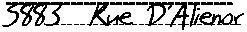
\includegraphics{crnn/generated/83}
				\caption[Generated images]{Examples of text generated by our tool. Dates, license plates and numbers are generated randomly according to different formats, whereas the others are sampled from various corpora. Names are not real, but randomly matchd between common first and last names.}
				\label{fig:generated_images}
			\end{figure}

		%........................................................................................
		\subsubsection*{Datasets}
			Equipped with the powerful tool above, we generate a corpus of size similar to RIMES (50\,000 training examples, \ds{Gen_50k}) using a selection of 25 handwriting-style fonts (examples in \autoref{fig:generated_images}). This converged to a validation \CER{4.6} after seeing, interestingly, the same amount of training examples as RIMES-trained model (\(\approx 750\)k). We noticed that further training for about twice as long brings improvements to the validation word error rate (\(\approx -3.5\%\)) while the CER remains constant. This suggests that the LSTM picks up further subtleties in the language model. However, the results on \ds{Test} were slightly worse that previous best, at \CER{67.31}. Evaluating this model on RIMES data exposes a key observation: it does not generalise there, either, having \CER{75.8}. While we actually wanted this data to be different, we expected it to be an extension to RIMES dataset. Seeing it is not, we trained a model on both of them (\ds{Gen_50K_RIM}) which achieved a new low, with \CER{45.78}.

			\urldef{\vLetter}\url{https://www.vletter.com/help/about-vletter.html}
			We hypothesised that the sub-par performance of the generated data was due to the small variation of fonts compared to human handwriting. Therefore, we created a database of 900 cursive fonts, each being a customised version of a real person's handwriting\footnote{\vLetter}; 100 of them were kept for validation. The model trained on this, \ds{Gen_800f} is better than the initial one of generated-only data (\ds{Gen_50k}). However, it still does not caputre all natural features of handwriting, performing slightly worse than \ds{Gen_50k_RIM}. Increasing the dataset size to 1 million examples (\ds{Gen_1M}) further approaches the mixed data model. Surprisingly, doubling the input resolution proves counterproductive (\ds{Gen_1M_64}).

		%........................................................................................
		\subsubsection*{Outcome}
			\begin{table}
				\centering
				\begin{tabular}{| l | *{4}{c |}}\hline
					\textbf{Dataset name} & \textbf{CER strict} & \textbf{CER lower} & \textbf{CER ascii} & \textbf{WER}\\\hline
					\ds{Gen_50k} & 67.31 & 63.67 & 63.44 & 93.82\\
					\ds{Gen_50k_RIM} & 45.78 & 42.06 & 42.13 & 85.78\\
					\ds{Gen_800f} & 49.02 & 43.98 & 43.66 & 86.21\\
					\ds{Gen_1M} & 46.06 & 39.85 & 39.55 & 83.62\\
					\ds{Gen_1M_64} & 50.24 & 43.29 & 42.97 & 85.06\\\hline
					(Best RIMES) & 60.58 & 57.71 & 57.71 & 94.83\\\hline
				\end{tabular}
				\caption[Generated datasets results]{Performance of models trained on different versions of generated datasets.}
				\label{tab:transcription_generated}
			\end{table}

			\begin{figure}
				\setkeys{Gin}{width=.3\linewidth}
				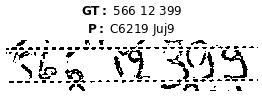
\includegraphics[valign=c]{crnn/gen_model_2}\hspace{5mm}
				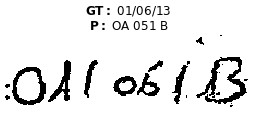
\includegraphics[valign=c]{crnn/gen_model_1}\hspace{5mm}
				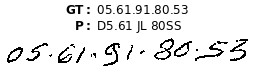
\includegraphics[valign=c]{crnn/gen_model_3}
				\caption[Understandably wrong predictions (1)]{A model trained on \ds{Gen_1M} makes wrong predictions on \ds{Test} dataset. However, examining them character by character, we realise they are not so off from what is shown in the image. For example, in the middle image the ``\texttt{0}'' is taken for an ``\texttt{O}'', the ``\texttt{1}'' really resembles ``\texttt{A}'', ``\texttt{/}'' character does look like a slanted ``\texttt{1}'' and the final ``\texttt{13}'' is undistinguishable from ``\texttt{B}''.
				}\label{fig:transcription_wrong}
			\end{figure}

			The series of experiments proved it is possible to learn relevant handwriting features and compensate for a small and uniform dataset (\autoref{tab:transcription_generated}).  However, significantly more data is needed to cover for the differences between natural and synthetic handwriting, in our case by a factor of 20. A mixed dataset seems to cover the best of both worlds, achieving the best performane at \CER{45.78}.

			Given that the results are still of no practical use, we inspected in more detail the generated data and the models' predictions. Looking at some examples in \autoref{fig:transcription_wrong}, we see that individual glyphs in the image actually correspond well to what the model predicts. The problem is that we, as humans, choose to interpret the whole differently than the concatenation of its parts. At the same time, parts derive their meaning from that of the whole. For example, glyphs that look like slanted bars are considered ones when grouped with another digit, but slashes when separating groups of digits, since we assume that the latter represents a date.

	%----------------------------------------------------------------------------------------

	\subsection{Corpus type}

		%... Description ........................................................................
			\urldef{\ICDAR}\url{http://u-pat.org/ICDAR2017/program_competitions.php}
			Based on the above observations, we try to address the shortcomings of the architecture. Specifically, we believe the LSTM language model suffers from the wild differences in the format of data, e.g.\ dates versus names. To the best of our knowledge, no good results have been published on such highly heterogeneous data. For example, the old problem of MNIST handwriting recognition is only concerned with digits, possibly arranged into strings. Additionally, the documents in ICDAR handwriting recognition competitions\footnote{\ICDAR} contain text from archaic documents which presents complex glyphs but still use normal language. Therefore, we try to split the challenge into smaller, more homogeneous sub-problems. However, instead of doing this manually, we will only provide information about the type of corpus that a given text belongs to and let the architecture learn and switch between different formats.

			To accomplish the above, we group the data into logical corpora which represent their type, or context. For the final pipeline, we envision that the assignment of text to a given corpus happens at detection time, where its location on the page can provide strong hints in this regard. Therefore, the categories are as follows:
			\begin{description}
				\item[Person names\vspace{-1.5em}]

				\item[Numbers] These are mostly phone numbers, but include, in general, any string of digits. We note that in real data some of these can also contain one or two characters, as they represent the contract ID.

				\item[Dates] These can come under a variety of formats, such as \texttt{27/04/03} and \texttt{22 Mar 2013}, with many possible delimiters. We group them all into the same category.

				\item[Hours] Similarly to dates, there are many possible formats for these as well.

				\item[Addresses] An address usually comprises of several parts: number, street, post code and city. In the statements, these are usually split in groups of two, over two lines. As such, address format usually follows a strict rule: ``\texttt{<digits>, <letters and spaces>}''.

				\item[License plates] These come in two formats which, unfortunately, are very different from one another: the new one is ``\texttt{AA 111 AA}'', while the old one is ``\texttt{1111 AAA 11}''.

				\item[Observations] This can include any natural language observations, makes and models of cars, country names, etc.
			\end{description}
			Although the formats are still not completely separated, most of them are well defined and have to be chosen from a smaller pool.

		%........................................................................................
		\subsubsection*{Strategy 1: preconditioning the LSTM}
			A body of work that is similar to our task was done in the area of image captioning. Most architectures there are also made up from a CNN feature extractor and an RNN language model, but the exact implementation details can have large influences on the result. For a first trial, we follow the implementation of \citet{lstm_precondition}, who precondition the LSTM by setting its hidden state to an encoding of the last convolutional feature map. Then they input and predict word vectors.

			We use a similar approach for providing the corpus information alongside the image features. We encode corpus class into an indicator vector \(\mathbbm{1}(c = 1) \in \{0, 1\}^F\), where \(F\) is the LSTM input size and \(c\) the unique integer ID of the corpus\footnote{This encoding scheme is also known as \emph{one-hot} encoding, in a vector of size \(F\)}. We use this as the first item in the features sequence, thus providing the same hidden state initialisation for all images belonging to the same corpus.

			We generate a new dataset as above, this time also keeping its origin information as corpus ID. A model trained on this, \ds{Gen_corpus_pre}, comes close to previous best, at \CER{47.94}. However, it does not improve on it. We believe there are two reasons behind this: first, the corpus feature vector is mostly filled with zeros when projected in image space, since there are just 7 different corpora and \(F = 512\) image features; second, our sequences are two to three times longer than those in image captioning, and not even the LSTM architecture can keep context for so long.

		%........................................................................................
		\subsubsection*{Strategy 2: add extra features}
			To overcome the problem of a very long sequence, we add the corpus information as extra features to the LSTM input, at all time steps. This is encoded as before, in an indicator vector \(\mathbbm{1}(c = 1) \in \{0,1\}^7\) (now only of necessary width), and is concatenated to the image features \(\mathcal{F}_t\) of each time step in the sequence\footnote{\todo{Use concatenation operator}}:\[
				\mathcal{F}'_t = \mathcal{F}_t \circ \mathbbm{1}(c = 1).
			\]

			Since the previous dataset already contains corpus information, we reuse it for training a new model with this configuration, \ds{Gen_corpus_all}. It achieves a new best, at \CER{41.76}. We observe it correctly learns formats of corpora, such as always predicting long numbers in groups of two digits, despite the ground truth being without white space.


		%........................................................................................
		\subsubsection*{Outcome}
			\begin{table}
				\centering
				\begin{tabular}{| l | *{4}{c |}}\hline
					\textbf{Dataset name} & \textbf{CER strict} & \textbf{CER lower} & \textbf{CER ascii} & \textbf{WER}\\\hline
					\ds{Gen_corpus_pre} & 47.94 & 40.75 & 40.44 & 81.82\\
					\ds{Gen_corpus_all} & 41.76 & 37.03 & 36.70 & 81.11\\\hline
					(Best generated) & 46.06 & 39.85 & 39.55 & 83.62\\\hline
				\end{tabular}
				\caption[Corpora information results]{Performance of a \CRNN{} model trained on a generated dataset of 1 million examples which include information about corpus of origin.}\label{tab:transcription_corpus}
			\end{table}

			Our hypothesis about the heterogeneity of data was validated and we sucessfully decrease it by bringing extra information into the architecture. However, the exact implementation makes a big difference, since the sequences we feed into the LSTM can be very long.

			\begin{figure}
				\begin{subfigure}[b]{.3\linewidth}
					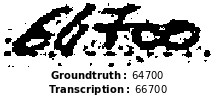
\includegraphics{crnn/cor_model_2}
					\caption{}\label{fig:cor_model_2}
				\end{subfigure}
				\begin{subfigure}[b]{.3\linewidth}
					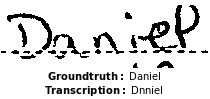
\includegraphics{crnn/cor_model_1}
					\caption{}\label{fig:cor_model_1}
				\end{subfigure}
				\begin{subfigure}[b]{.3\linewidth}
					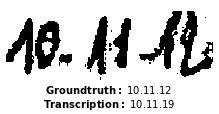
\includegraphics{crnn/cor_model_3}
					\caption{}\label{fig:cor_model_3}
				\end{subfigure}
				\caption[Understandably wrong predictions (2)]{A model trained with knowledge about the type of text it sees understands better the format of different strings, e.g.\ in \subref{fig:cor_model_3} it completes the second dot by itself. However, it still strugles to make sensible choices, like in the case of \subref{fig:cor_model_2}. There, the second digit coult be taken for a ``\texttt{6}'', if it were on its own; but seeing the first glyph is an actual ``\texttt{6}'' gives us an indication that the second cannot be the same thing.}\label{fig:corpus_wrong}
			\end{figure}
			We again inspect in detail the type of mistakes that the model is making (\autoref{fig:corpus_wrong}) and observe that these are mostly related to the path that the model finds through the activations matrix. Specifically, the approximation in \autoref{sec:CTC} makes it predict the character of maximum activation. For example, for the last digit in \autoref{fig:cor_model_3} is an unusual ``\texttt{2}'' that \emph{does} have a part looking like a regular ``\texttt{9}''; this part probably overlaps maximally with the model's representation of ``\texttt{9}'' and that is what the model predicts.

	%----------------------------------------------------------------------------------------

	\subsection{Elastic deformations}
		%... Description ........................................................................
			Despite using over 800 realistic handwriting fonts for generating data, and affine transformations on top such as slanting and skewing, we observed even the best models still do not capture all the variation in natural handwriting. This pointed us to the advice of \citet{elastic_distortions}, who describe a method of data augmentation for handwritten digits. Specifically, they propose using random displacement fields \(\Delta \ve{x}, \Delta \ve{y} \in \operatorname{rand}(-1,1)\) which correspond to uncontrolled oscillations of the hand muscles, dampened by inertia. These are then used as parameters of an interpolation for sampling in the original image. However, using the purely random values results in a noisy distortion of the image. This can be accommodated by first convolving the fields \(\Delta \ve{x}, \Delta \ve{y}\) with a Gaussian kernel of standard deviation \(\sigma\), which becomes the elastic coefficient. Seeing that small values of sigma produce too much deviation (\autoref{fig:elastic_4}), we select sigma from a normal distribution \(\mathcal{N}(8, 2)\), but threshold it at values bigger than 5. Another important parameter is \(\alpha\) which controls the displacement amount. While the authors recommend a hard value of \(\alpha=34\), we found this to be dependent on the image size. Therefore, we empirically determined a good relation to be \(\alpha = 1.5 \times H\), where \(H\) is the height of the image.
			\begin{figure}
				\begin{subfigure}[t]{.32\linewidth}
					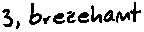
\includegraphics{crnn/elastic}
					\caption{Original image}\label{fig:elastic_0}
				\end{subfigure}
				\begin{subfigure}[t]{.32\linewidth}
					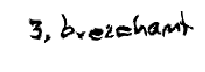
\includegraphics{crnn/elastic4}
					\caption{\(\sigma = 4\)}\label{fig:elastic_4}
				\end{subfigure}
				\begin{subfigure}[t]{.32\linewidth}
					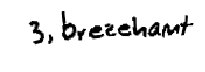
\includegraphics{crnn/elastic8}
					\caption{\(\sigma = 8\)}\label{fig:elastic_8}
				\end{subfigure}
				\caption[Elastic deformations]{Examples of influence of the elastic coefficient \(\sigma\)}
			\end{figure}

		%........................................................................................
		\subsubsection*{Datasets and outcome}
			We enhanced the generator from \autoref{sec:generator} to include this type of deformations as well, and, as before, we produced a dataset of 1 million examples, with corpus information included, \ds{Gen_elastic}. We observed from the start a much better performance on the validation dataset, compared to the previous best model, \ds{Gen_corpus_all} (\autoref{fig:elastic_cer_drop}). However, this does not readily transfer to the \ds{Test} dataset, as it attains a \mbox{\CER{42.2}} that is close to the one before. Moreover, we let this model train for much longer than any previous ones and observe that although its \emph{validation} performance remains stable, at a given point it starts to perform worse on \ds{Test}(\autoref{tab:elastic_corpus}). It is important to note that this type of overfit cannot be detected during training since we do not validate on \ds{Test}. Therefore, the model is picking up very subtle features which differentiate generated data from real one, although for us both look the same.

			\begin{figure}
				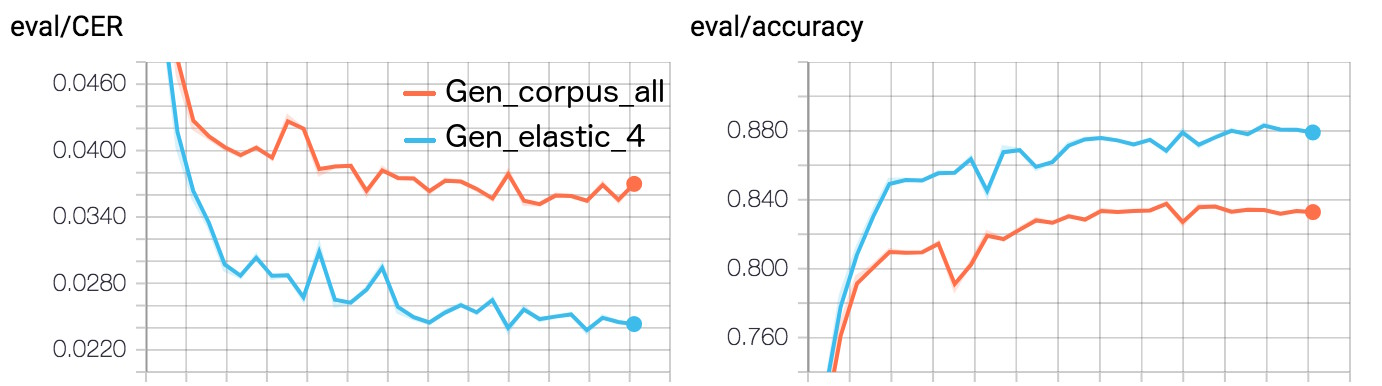
\includegraphics{crnn/elastic_drop}
				\caption[Improvements of elastic deformations]{The curves show the training evolution of validation CER and accuracy \mbox{(\(= 1 - \wer\))} of the best models with (blue) and without (orange) elastic deformations.}\label{fig:elastic_cer_drop}
			\end{figure}

			\begin{table}
				\centering
				\begin{tabular}{| l | *{5}{c |}}\hline
					\textbf{Dataset name} & \textbf{epochs} & \textbf{CER strict} & \textbf{CER lower} & \textbf{CER ascii} & \textbf{WER}\\\hline
					\ds{Gen_elastic_1}    &  8 & 45.14 & 38.59 & 38.30 & 83.33\\
					\ds{Gen_elastic_2}    & 18 & 43.97 & 38.95 & 38.70 & 82.90\\
					\ds{Gen_elastic_3}    & 31 & 42.20 & 36.92 & 36.64 & 81.68\\
					\ds{Gen_elastic_4}    & 48 & 45.29 & 40.16 & 39.89 & 83.41\\\hline
					(Best ``with-corpus'')& 31 & 41.76 & 37.03 & 36.70 & 81.11\\\hline
				\end{tabular}
				\caption[Elastic deformation results]{Performances obtained when training on a corpus with elastic deformations included, at different training times.
				}\label{tab:elastic_corpus}
			\end{table}


%========================================================================================

\section{Results}\label{sec:transcription_results}
	\begin{table}
		\centering
		\begin{tabular}{| l | *{4}{c |}}\hline
			\textbf{Dataset name} & \textbf{CER strict} & \textbf{CER lower} & \textbf{CER ascii} & \textbf{WER}\\
			\hline
			\ds{Word} & 115.52 & 109.98 & 109.83 & 98.28\\
			\ds{Word_bin} & 62.43 & 59.44 & 59.43 &\bf 94.25\\
			\ds{Word_bin_drop} &\bf 60.58 &\bf 57.71 &\bf 57.71 & 94.83\\
			\ds{Word_short_IAM} & 104.19 & 100.24 & 100.15 & 98.78\\
			% \ds{Word_short} & 103.70 & 100.97 & 100.74 & 98.71\\
			\ds{Word_short_drop} & 103.77 & 100.36 & 100.17 & 97.70\\
			\hline

			\ds{Gen_50k} & 67.31 & 63.67 & 63.44 & 93.82\\
			\ds{Gen_50k_RIM} & 45.78 & 42.06 & 42.13 & 85.78\\
			\ds{Gen_800f} & 49.02 & 43.98 & 43.66 & 86.21\\
			\ds{Gen_1M} &\bf 46.06 &\bf 39.85 &\bf 39.55 &\bf 83.62\\
			\ds{Gen_1M_64} & 50.24 & 43.29 & 42.97 & 85.06\\
			\hline

			\ds{Gen_corpus_pre} & 47.94 & 40.75 & 40.44 & 81.82\\
			\rowcolor{LightGreen}
			\ds{Gen_corpus_all} &\bf 41.76 &\bf 37.03 &\bf 36.70 &\bf 81.11\\
			\hline

			\ds{Gen_elastic_1} & 45.14 & 38.59 & 38.30 & 83.33\\
			\ds{Gen_elastic_2} & 43.97 & 38.95 & 38.70 & 82.90\\
			\ds{Gen_elastic_3} &\bf 42.20 &\bf 36.92 &\bf 36.64 &\bf 81.68\\
			\ds{Gen_elastic_4} & 45.29 & 40.16 & 39.89 & 83.41\\
			\hline\hline
			\ds{Test \footnotesize{(600 examples)}} & 21.59 & -- & -- & 62.11\\
			\hline
		\end{tabular}
		\caption[All transcription results]{Performances of different models. \textbf{Bold} entries are the best in their category, while the \colorbox{LightGreen}{highlighted} entry is the best overall.
		}\label{tab:transcription_results}
	\end{table}


	% corpus_all and elastic_3 are very close for lower

	We summarise the results of our experiments in \autoref{tab:transcription_results}. We see that large amounts of generated data overcome the limitations of a uniform dataset such as RIMES and that adding contextual information such as corpus type helps the architecture build better language models. However, the generated data does not bring benefits as big as it does in OCR and printed text recognition. We believe this is expected due to a number of reasons. First, printed text is usually put on a hard support; therefore all images of such text represent just an affine transformation of the original. This is in contrast to handwritten text which presents many subtle variations at stroke level. Then, text-in-the-wild usually comprises of words and language; with a little effort we can generate all such possible instances. In contrast, our task has to cope with almost infinite combinations of digits and letters. Finally, fonts used for printed text have unambiguous glyphs, in general; apart from \{\texttt{i,1,l}\}, all glyphs are intentionally very different from one another. However, in handwritting, the same glyph can correspond to different characters and only context can solve the ambiguity.

	We also observe that the architecture overfits to generated data, despite the large number of fonts and the elastic deformations. This, again, makes the task easier for printed text, since virtually all of it was generated by an existing font, unlike handwriting which is almost unique to every person.

	Finally, we tried to explore the maximum capabilities of the current transcription system by fine-tuning the best model on a subset of \ds{Test} dataset. Using 800 text examples for training and 600 for testing, we managed to improve the performance up to \mbox{\CER{21}}, \WER{62}. Unfortunately, we do not have a human level error rate to compare with. Also, it is unclear whether more training data would be beneficial or a more powerful architecture is needed for further improvements.

